\documentclass[12pt,a4paper,english]{paper} 
\usepackage{fontspec}
\usepackage[utf8]{inputenc}
\usepackage[left=0.65in,right=0.65in,top=2cm,bottom=1in]{geometry}
\usepackage{multirow}
\usepackage{hyperref}
\usepackage{graphicx}
\usepackage{bm}
\usepackage[usenames,dvipsnames]{color}
\usepackage{booktabs}
\usepackage[inline]{enumitem}
\usepackage{fancyhdr}
\usepackage[most]{tcolorbox}
\usepackage{changepage}
\usepackage[square,sort,comma,numbers]{natbib}
\usepackage{amsmath}
\usepackage{amssymb}
\usepackage{eucal}
\usepackage[]{minted}
\usepackage{latexsym}
\usepackage{indentfirst}
\usepackage[ruled,vlined]{algorithm2e}
\usepackage[english]{babel}
\usepackage[autostyle, english = american]{csquotes}
\usepackage{paralist}
\setlist[itemize]{noitemsep, topsep=0pt}
\MakeOuterQuote{"}

\def \courseNumber {CS6600}
\def \courseName {Computer Architecture}
\def \assignmentName {Tournament Branch Predictor}
\def \myName {Arjun Menon V, Akilesh Kannan}
\def \rollNumber {EE18B104, EE18B122}

\setlength{\headheight}{14pt}

\pagestyle{fancy}
\fancyhf{}
\rhead{\assignmentName}
\lhead{\courseNumber: \courseName}
\cfoot{\thepage}

% \linespread{1.2}

\renewcommand{\familydefault}{\sfdefault} %command to change font to sans-serif

\definecolor{blue(ryb)}{rgb}{0.01, 0.28, 1.0}
\definecolor{green(ryb)}{rgb}{0.28, 1.0, 0.01}
\definecolor{red(ryb)}{rgb}{1.0, 0.01, 0.28}
\definecolor{black(ryb)}{rgb}{0, 0, 0}
\definecolor{gray(ryb)}{rgb}{0.75, 0.75, 0.75}
\definecolor{orange}{RGB}{255,155,0}
\definecolor{formalblue}{rgb}{0.95,0.95,1}
\definecolor{formalred}{rgb}{1,0.95,0.95}

\newenvironment{colorboxed}[4][gray]{
\begin{tcolorbox}[colback=#1!3!white,colframe=#1(ryb)!50!black,title=\textbf{#2 #3},#4]
}{
\end{tcolorbox}
}

\newenvironment{warning}{%
  \def\FrameCommand{%
    \hspace{1pt}%
    {\color{red}\vrule width 2pt}%
    {\color{formalred}\vrule width 4pt}%
    \colorbox{formalred}%
  }%
  \MakeFramed{\advance\hsize-\width\FrameRestore}%
  \noindent\hspace{-4.55pt}% disable indenting first paragraph
  \begin{adjustwidth}{7pt}{}%
  \vspace{2pt}\vspace{2pt}%
}
{%
  \vspace{2pt}\end{adjustwidth}\endMakeFramed%
}

\newenvironment{results}{%
  \def\FrameCommand{%
    \hspace{1pt}%
    {\color{blue}\vrule width 2pt}%
    {\color{formalblue}\vrule width 4pt}%
    \colorbox{formalblue}%
  }%
  \MakeFramed{\advance\hsize-\width\FrameRestore}%
  \noindent\hspace{-4.55pt}% disable indenting first paragraph
  \begin{adjustwidth}{7pt}{}%
  \vspace{2pt}\vspace{2pt}%
}
{%
  \vspace{2pt}\end{adjustwidth}\endMakeFramed%
}

\begin{document} 
\thispagestyle{empty}
\vspace{-4.5cm}

\hspace*{-\parindent}
\begin{minipage}{0.65\textwidth}
\fontsize{22pt}{10pt}\selectfont\textbf{\assignmentName}\\[1mm]
\Large
\textit{\courseNumber: \courseName}\\[5mm]
\Large \myName \\[1mm]
\normalsize \rollNumber \\
\end{minipage}\hfill% push everything to the right
\raisebox{-13mm}{
\includegraphics[scale=.28]{logo.pdf}}

\hrule \hrule
\medskip

\begin{warning}
The code developed for this assignment can be found here - \href{https://github.com/aklsh/TournamentBPU}{link}
\end{warning}

\section{Introduction}
Architecture techniques that exploit Instruction-Level Parallelism, such as Pipelining and Superscalar execution, are often adversely affected by stalls in the pipeline due to branch instructions. With branch instructions forming a significant portion of a typical program, it is imperative to use effective dynamic (run-time) branch prediction mechanisms to make the most out of ILP.

In this assignment, we implement the Tournament Branch Predictor \cite{mcfarling_combining_1993} using the framework provided by JILP for the 2016 version of the Branch Prediction Championship (CBP2016). A quick summary of some popular dynamic branch prediction ideas is provided leading up to the Tournament Predictor. 

\subsection{4-state FSM based Predictor}
A four-state Finite State Machine is used to predict the branch direction based on the past history of branch directions that were taken. The states \texttt{00} and \texttt{11} correspond to a strong prediction of \texttt{NOT-TAKEN} and \texttt{TAKEN} respectively- the predicted direction is changed only after at least two consecutive incorrect decisions. The local and global predictors in the Tournament Predictor use $n$-bit ($2^n$ state) FSM based predictors (in our implementation, we use $n=2$).
\begin{figure}[H]
    \centering
    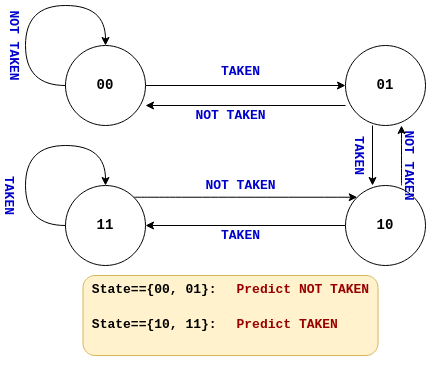
\includegraphics[scale=0.5]{4stateFSM.png}
    \caption{4-state FSM based Predictor. Text in blue indicates the true branch direction as determined in the execution stage of the pipeline}
\end{figure}

\subsection{Correlating Branch Predictor}
Often, the branch results of instructions with similar branch history are correlated. To account this behaviour in the prediction mechanism, a correlating branch predictor extends the FSM-based predictor by maintaining multiple FSM counters for different branch histories. Branch instructions with the same branch history share the FSM state. To facilitate this, a table of branch histories, indexed by the branch instruction address, is maintained with each entry containing the branch history of the instructions mapped to it. Since the History Table size is limited, only a few bits from the PC is required to index the table.

When there is only one entry in the history table, the correlating predictor essentially tracks global prediction history. With sufficiently large history tables, each FSM in the correlating predictor uses local branch history information to make the decision.

\subsection{The Tournament Branch Predictor \cite{mcfarling_combining_1993}}
Different programs exhibit varying trends in the correlation between branch instructions- some functions may have a high correlation in the global branch history while some others may exhibit correlation locally. This trend may even vary in the same program. A tournament branch predictor integrates a global correlating predictor with a local correlating predictor. This lets the prediction mechanism adapt to the program's correlation trend dynamically.

When both the local and global predictors agree on a prediction, the prediction is used, else the tournament predictor uses yet another FSM (choice predictor) to choose between the local predictor and the global predictor. The choice predictor uses a 4-state FSM similar to the one discussed. When the choice predictor's state is equal to \texttt{00} or \texttt{01}, the local predictor is chosen, else the global predictor is chosen. Upon resolution of the branch direction, the state of the FSM is updated in the direction favouring the correct predictor.
\begin{figure}[H]
    \centering
    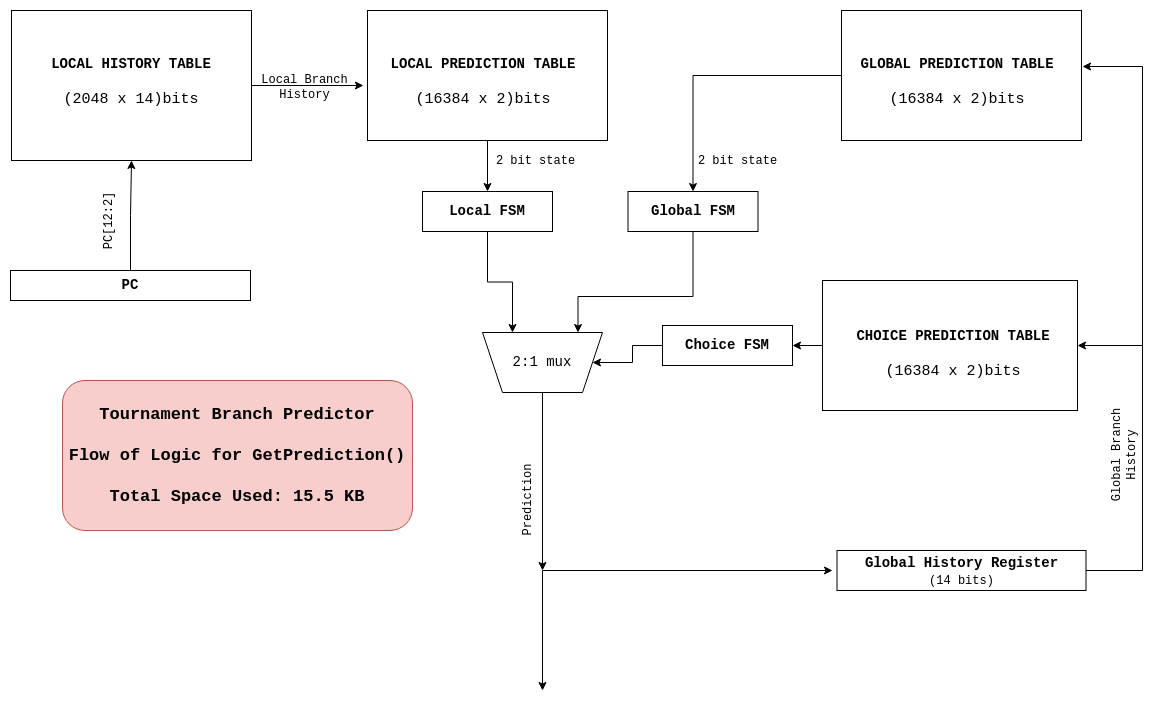
\includegraphics[scale=0.35]{TourBP.png}
    \caption{Tournament Branch Predictor}
\end{figure}
\subsubsection{Storage Budget Justification}
\begin{table}[H]
\centering
\begin{tabular}{|c|c|c|c|}
\hline
\textbf{Structure} & \textbf{Number} & \begin{tabular}[c]{@{}c@{}}\textbf{Size/structure}\\ \textbf{(in bits)}\end{tabular} & \textbf{Total Size (in bits)} \\ \hline
\multicolumn{4}{|c|}{\textit{Global Predictor}}    \\ \hline
GHR           & 1      & 14 & 14          \\ \hline
GPT counters  & 16384  & 2  & 32678 (32K) \\ \hline
\multicolumn{4}{|c|}{\textit{Local Predictor}}     \\ \hline
LHT entry     & 2048   & 14 & 28672 (28K) \\ \hline
LPT counters  & 16384  & 2  & 32768 (32K) \\ \hline
\multicolumn{4}{|c|}{\textit{Choice Predictor}}    \\ \hline
CPT counters  & 16384  & 2  & 32768 (32K) \\ \hline
\multicolumn{3}{|c|}{Total} & 124K + 14 $\approx$ 15.5KB  \\ \hline
\end{tabular}
\caption{Storage allocation}
\end{table}

$\%$ Used out of maximum allowed budget (16KB) = $96.88\%$

\section{Code Structure - \texttt{class PREDICTOR}}
A data structure given by the framework, with the following fields and methods to help in designing the branch predictor. 
\subsection{Methods}
    \begin{compactitem}
        \item \texttt{PREDICTOR()}: Constructor to initialise the tables, \texttt{GHR} and counters.
        \item \texttt{\textasciitilde PREDICTOR()}: Destructor to delete all dynamically allocated pointers.
        \item \texttt{GetPrediction()}: Takes as input the \texttt{PC} value corresponding to the branch instruction, and returns \texttt{TAKEN} (\texttt{True}) or \texttt{NOT-TAKEN} (\texttt{False}).
        \item \texttt{UpdatePrediction()}: Takes as input the \texttt{PC}, predicted direction of branch (\texttt{predDir}) and true direction of the branch (\texttt{resolveDir}) and updates the \texttt{GHR}, local history, local predictor counter, global predictor counter and the choice predictor counter that were used to predict the direction.
    \end{compactitem}
\subsection{Fields}
    \subsubsection{Global Predictor Related}
    \begin{compactitem}
        \item \texttt{ghr}: Global History Register
        \item \texttt{gpt}: Global Predictor Table
        \item \texttt{numGptEntries}: Number of entries in the GPT
    \end{compactitem}

    \subsubsection{Local Predictor Related}
    \begin{compactitem}
        \item \texttt{lht}: Local History Table
        \item \texttt{numLhtEntries}: Number of entries in the LHT
        \item \texttt{lpt}: Local Predictor Table
        \item \texttt{numLptEntries}: Number of entries in the LPT
    \end{compactitem}

    \subsubsection{Choice Predictor Related}
    \begin{compactitem}
        \item \texttt{cpt}: Choice Predictor Table
        \item \texttt{numCptEntries}: Number of entries in the CPT
    \end{compactitem}
    
\section{Results}
We had experimented with the initial choice in the choice predictor to observe how the initial bias of the choice predictor affected the overall outcome of the BPU. In one configuration, we started all the counters with a \textit{Weakly Local Bias} (\texttt{01}) and in the other, a \texttt{Weakly Global Bias} (\texttt{10}).

\begin{figure}[H]
    \centering
    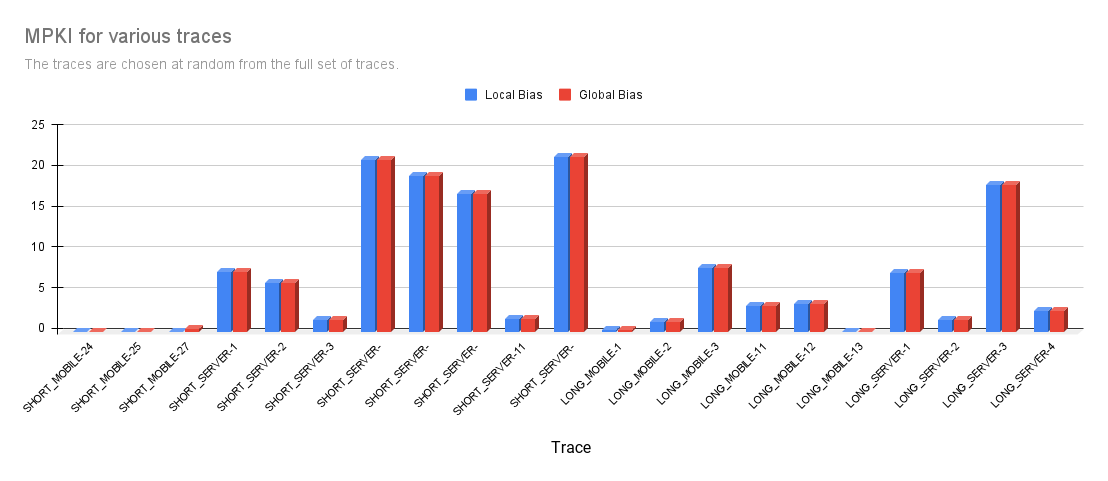
\includegraphics[scale=0.4]{MPKI for various traces.png}
    \caption{MisPrediction per 1K Instructions}
\end{figure}
\begin{figure}[H]
    \centering
    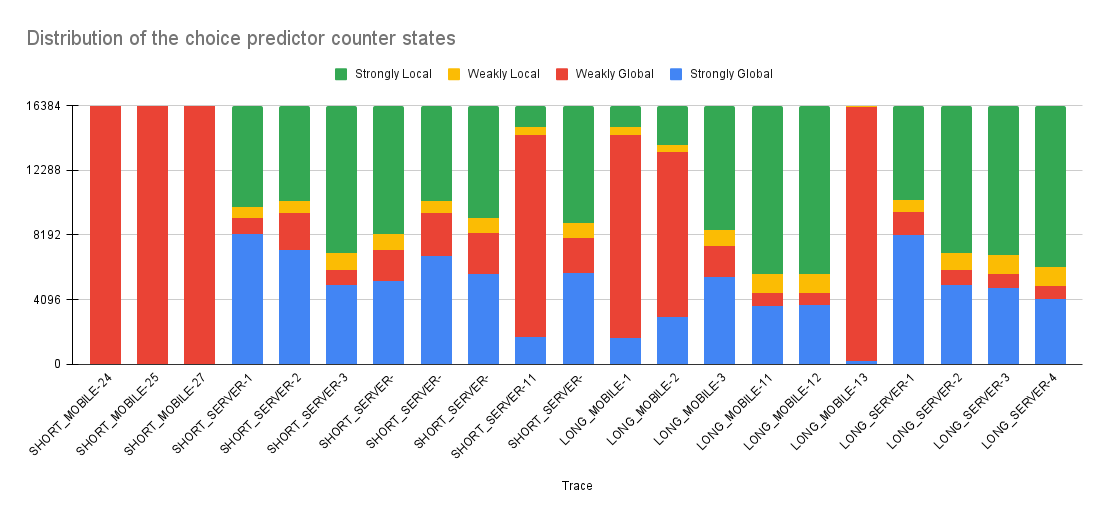
\includegraphics[scale=0.4]{Distribution of the choice predictor counter states_Global.png}
    \caption{Choice Distribution with Global Bias}
\end{figure}
\begin{figure}[H]
    \centering
    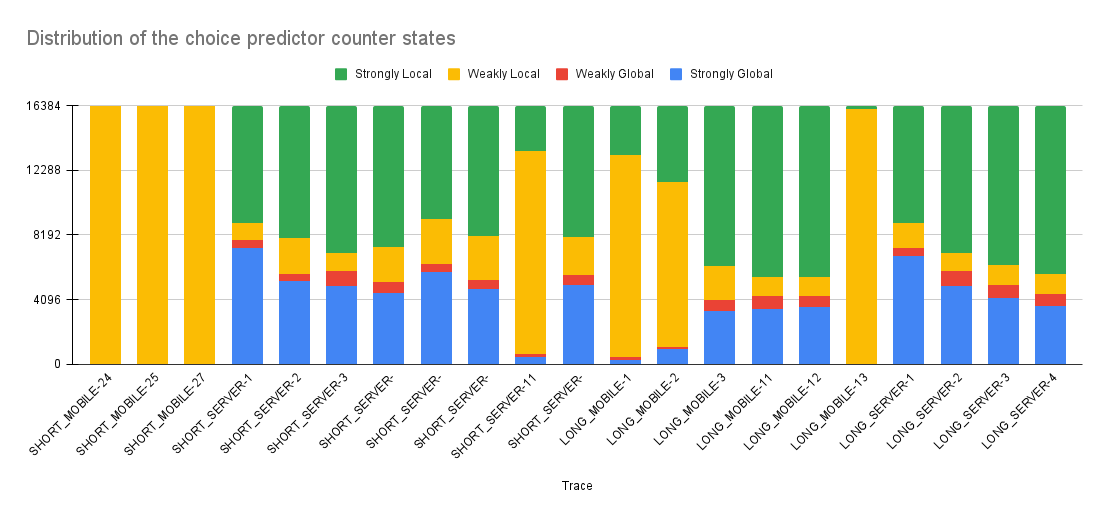
\includegraphics[scale=0.4]{Distribution of the choice predictor counter states_Local.png}
    \caption{Choice Distribution with Local Bias}
\end{figure}
\begin{figure}[H]
    \centering
    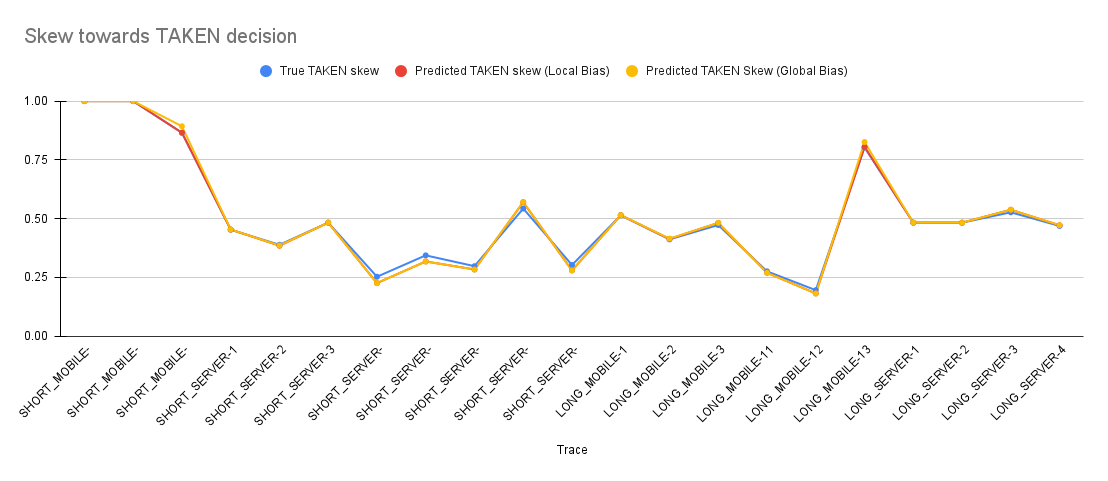
\includegraphics[scale=0.4]{Skew towards TAKEN decision.png}
    \caption{Skew towards \texttt{TAKEN} branches}
\end{figure}

We can see that the MPKI doesn't change much between the two configurations. This is expected because we don't expect the initial bias of the choice predictor to affect the steady state misprediction rate.

However, we can clearly see that the bias does affect the choice predictor's decisions. A global bias would make the predictor choose the global predictor more often and vice-versa. This happens only if the choice predictor isn't very confident about it's prediction, i.e., it produces a \textit{weak} prediction. If the prediction is \textit{strong}, then the initial bias doesn't play a role. We can see the same in the plots too - the \textit{strong} predictions remain the same, while the \textit{weak} ones are interchanged.

%Beginning References. Don't add any text beyond this.
%------------------------------------------

%\newpage %sending References to the last page

\bibliography{references}
\bibliographystyle{acm}
\end{document}
